
\documentclass{article}
\usepackage[left=2cm,right=2cm,top=3cm,bottom=3cm,letterpaper]{geometry}
\usepackage[spanish]{babel}
\usepackage[utf8]{inputenc}

\usepackage{verbatim, array}
\usepackage{hyperref}
\usepackage{amsmath, amsfonts, amssymb}
\usepackage{graphicx}
\usepackage[T1]{fontenc}

\newcommand{\jimage}[3]{\begin{figure}[h!]\includegraphics[width=#1\textwidth]{#2}\caption{#3}\end{figure}\vskip10pt}
\newcommand{\jcimage}[3]{\begin{figure}[h!]\centering\includegraphics[width=#1\textwidth]{#2}\caption{#3}\end{figure}\vskip10pt}

\author{Héctor Enrique Gómez Morales}
\title{Análisis y mejoras en el procesamiento de imágenes obtenidas por Resonancia Magnética Funcional: Resting State, Contraste BOLD.}
\date{15 de junio de 2015}
\begin{document}
%\maketitle
\section{Introducción}

La técnica de imagen por resonancia magnética es una técnica de diagnóstico que tiene como ventaja con respecto a la tomografía axial computada el que no es invasiva y tiene mayor contraste para tejidos blandos. Esta técnica hace uso del concepto físico de resonancia magnética, dónde los protones del átomo de hidrógeno de la estructura a estudiar son sometidos a un campo magnético estático de alta intensidad (aproximadamente 60 000 veces mayor que el campo magnético terrestre) a partir del cual se imprime un pulso de radiofrecuencia de la frecuencia de Larmor para que dichos protones emitan un señal la cuál es medida por las antenas del aparato en el eje x a partir de las cuál se reconstruyen imágenes tridimensionales de la estructura de interés que son interpretadas posteriormente por los médicos radiólogos.

En el proceso de obtención, post procesamiento y análisis de las imágenes de resonancia magnética cerebrales intervienen profesionales de varias disciplinas como son médicos, psicólogos, especialistas en neurociencias, ingenieros, físicos, estadistas, computológos, etc.

El papel de la computación es vital en la reconstrucción de las imágenes a partir de la información obtenida por el resonador y en el análisis posterior de las imágenes reconstruidas.

La Resonancia Magnética Funcional (\textbf{RMf}) es una técnica de neuroimagen que permite registrar la actividad cerebral en vivo. Provee una resolución espacial lo que la ha convertido en una técnica de neuroimagen por excelencia. 

\section{Objetivos}

\begin{itemize}
\item Comprender los principios fundamentales de la Imagenología por Resonancia Magnética.

\item Facilitar la instalación y configuración del software necesario para el procesamiento y análisis de las imágenes obtenidas por \textbf{RMf}.

\item Implementar programas para facilitar el preprocesamiento y análisis de las imágenes por \textbf{RMf}.

\item Analizar los programas \texttt{FCON1000} y \texttt{CPAC} para ver que tan factible es realizar extensiones para usar otro tipo de análisis, como \texttt{MELODIC}.

\item Apoyar en el almacenamiento y respaldo de las imágenes adquiridas.
\end{itemize}

\section{Desarrollo}
Durante el primer mes me enfoqué a realizar una investigación bibliográfica acerca de los principios básicos de la resonancia magnética. Haciendo énfasis en las técnicas de resonancia magnética funcional \textbf{RMf}, en particular estudiando el contraste \texttt{BOLD}[1], la cual detecta el cambio en la susceptibilidad magnética debido al nivel de oxigenación en la sangre.

En el segundo mes me enfoqué a aprender sobre las bibliotecas \texttt{FSL} (FMRIB Software Library) y \texttt{AFNI} (Analysis of Functional NeuroImages) que son el software más usado para realizar el preprocesamiento, análisis y visualización de imágenes.

Posteriormente implementé un programa \texttt{NeuroVagrant} que facilita la instalación del software de análisis para así obtener un entorno de desarrollo en el menor tiempo posible. Se hizo uso de \texttt{Vagrant}, \texttt{VirtualBox} y \texttt{NeuroDebian} para realizar la instalación y configuración de una máquina virtual con todo el software necesario para las necesidades de los proyectos que se tienen en el Instituto.

Los proyectos que se estaban implementando durante mi servicio fueron: \texttt{CONECTOMA} cuyo objetivo era la medición de conectividad en pacientes con adicción a la cocaína y \texttt{SCA7} para medir la conectividad en pacientes con ataxia cerebroespinal tipo 7. En ambos proyectos se obtuvieron secuencias funcionales del tipo DTI (\texttt{tensor de difusión}) y FE\_EPI (\texttt{resting state}).

Ayude en el preprocesamiento de las imágenes obtenidas de los proyectos \texttt{CONECTOMA} y \texttt{SCA7} cambiando las imágenes del formato \texttt{DICOM} (Digital Imaging and Communication in Medicine) al formato \texttt{NIFTI} para su análisis estadístico posterior. Implementé varios programas en \texttt{Bash} para convertir y construir la estructura de archivos necesaria para poder realizar su análisis estadístico.

Como parte del preprocesamiento implementé scripts para realizar la normalización de las imágenes, que consiste en ajustar la posición, la orientación y el tamaño de cada cerebro con un cerebro individual con un cerebro de referencia (\textbf{template}). También realicé la segmentación y suavizado de las imágenes todo esto para facilitar su análisis. 

Investigué la estructura interna y posibilidad de extensión de los programas \texttt{FCON1000} y \texttt{CPAC}. En particular buscaba extender alguno de estos dos programas para realizar análisis usando \texttt{MELODIC} (Multivariate Exploratory Linear Optimized Decomposition into Independent Components) que es una técnica que realiza análisis por componentes independientes (\texttt{ICA})[2].

Implementé un módulo de \texttt{CPAC} para realizar el análisis por medio de \texttt{MELODIC}

Finalmente implementé un conjunto de scripts para ayudar al almacenamiento y respaldo de las imágenes del resonador, tomando en cuenta las necesidades de seguridad y confidencialidad dado que se están manejando datos clínicos.

\section{Resultados y Conclusiones}

Se logró automatizar la instalación del ambiente de trabajo teniendo en cuenta las necesidades del departamento. Ahora se tiene un entorno de desarrollo totalmente funcional y listo para ser usado en pocas horas sin necesidad de la atención constante del usuario. Esto además permite el poder experimentar con nuevas herramientas, bibliotecas y programas dado que se puede reinstalar rápidamente el ambiente.

También se logró analizar alternativas para implementar \texttt{MELODIC}, se hizo la investigación de los programas \texttt{FCON1000} y \texttt{CPAC}. Se utilizó \texttt{CPAC} como base para realizar la implementación de un módulo 
que realiza el análisis por medio de \texttt{MELODIC}.

Además se implementó un conjunto de programas  para la manipulación, preproceso y respaldo de la las imágenes obtenidas del resonador, la realización del respaldo fue particularmente arduo por problemas con el sistema operativo (basado en Windows 7).

Se implementaron programas para realizar el preprocesamiento necesario para poder realizar un análisis por \textbf{ICA} usando \texttt{MELODIC}.

Finalmente tuve la oportunidad de observar la colaboración de científicos de diferentes disciplinas y pude corroborar la importancia de la comunicación para el desarrollo exitoso entre estas diferentes disciplinas.

\begin{figure}[h!]
	\centering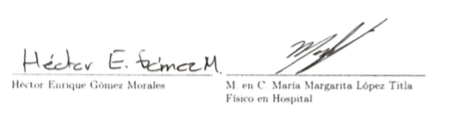
\includegraphics[width=0.7\textwidth]{signatures.png}
\end{figure}\vskip10pt

\section{Bibliografía}

[1] H.F. Scott and B.M. Feroze. Functional MRI: basic principles and clinical applications. Springer, 2006.

[2] F. Gregory Ashby, Statistical Analysis of FMRI Data, MIT Press, 2011.

\end{document}
